\documentclass[12pt]{article}
\usepackage{fullpage, tikz, graphicx}
\author{David Song}
\title{Problem Set 0 (Gov 2000)}
\date{September 12, 2019}
\begin{document}
\maketitle

\section*{Problem 1}
\begin{flushleft}
Mean of Democratic vote share: $\mu_{Dem} \approx 0.31479$

Mean of Republican vote share: $\mu_{Rep} \approx 0.63136$
\end{flushleft}

\section*{Problem 2}
\begin{center}
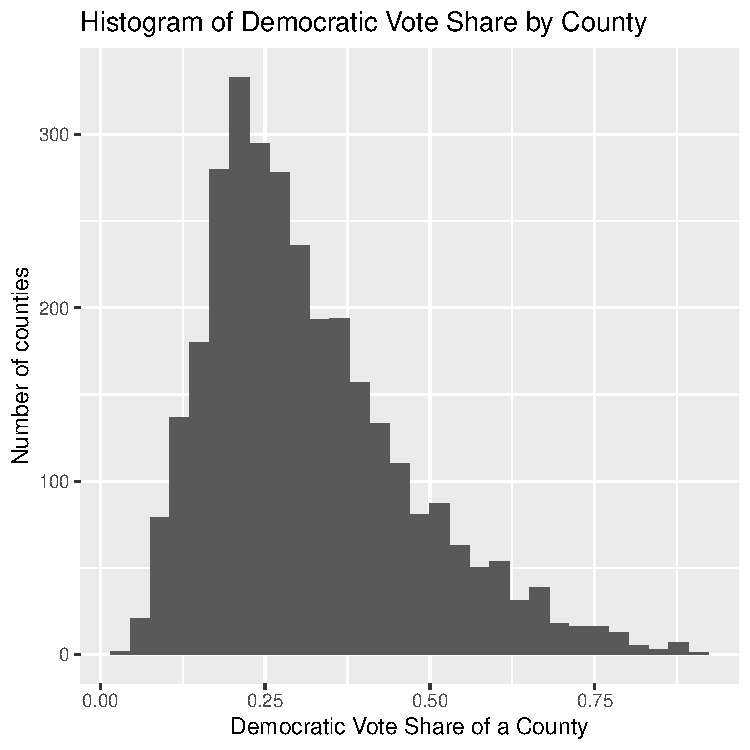
\includegraphics[width=0.4\textwidth] {HW0hist1}
\hspace{25pt}
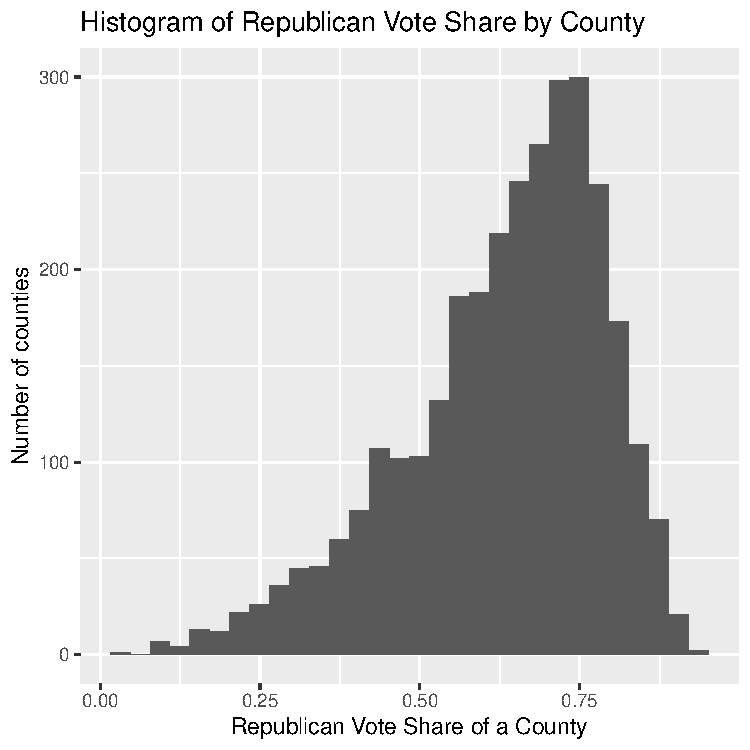
\includegraphics[width=0.4\textwidth] {HW0hist2}
\end{center}

\section*{Problem 3}
\begin{flushleft}
Nation-wide Democratic voter share: $\approx 0.4806$

Nation-wide Republican voter share: $\approx 0.4593$

No, they are not equal to the means of their county-level vote shares. This is because the means of county-level vote shares are not weighted for the size of the voting population in a county. For example, a small county that voted heavily Republican is weighted the same as a large county that voted heavily Democrat in Problem 2. 
\end{flushleft}

\section*{Problem 4}
\begin{center}
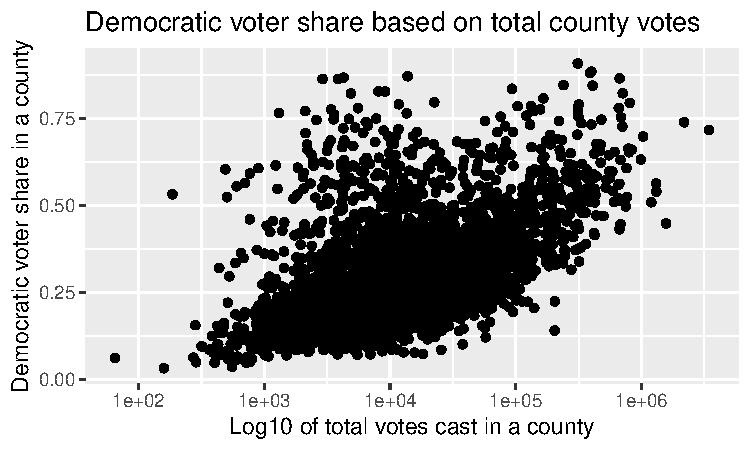
\includegraphics[width=0.7\textwidth] {HW0plot1}
\end{center}

There appears to be a relatively strong positive linear correlation between total number of voters and Democratic voter share in a county. 

In short, we can suggest that counties with a larger number of voters are more likely to have more Democratic voters than smaller counties. 

\section*{Problem 5}
County with largest third-party vote share: Los Angeles

\section*{Problem 6}
\begin{center}
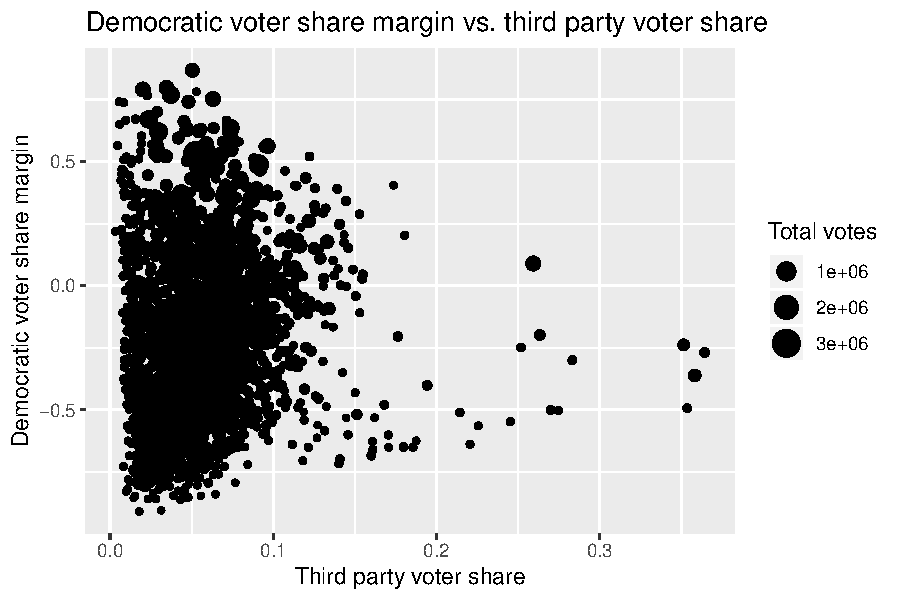
\includegraphics[width=0.7\textwidth] {HW0plot2}
\end{center}
\begin{flushleft}
In general, when total third party voter share is less than 10\%, there appears to be no relationship between third party voter share and Democratic voter share margins.

In contrast, at higher third party voter shares, there seems to be a negative correlation between third party voter share and Democratic voter share margins. 
This possibly suggests that in counties with more third party voters, Democrats were more likely to lose against Republicans (i.e. have negative voter share margins).

\end{flushleft}
\end{document}
